\documentclass[review]{elsarticle}

\usepackage{lineno}
\usepackage[hidelinks]{hyperref}
\usepackage{pdflscape}
\modulolinenumbers[5]

% \journal{Geochemica and Cosmochemica Acta}
\journal{no one yet}

%%%%%%%%%%%%%%%%%%%%%%%
%% Elsevier bibliography styles
%%%%%%%%%%%%%%%%%%%%%%%
%% To change the style, put a % in front of the second line of the current style and
%% remove the % from the second line of the style you would like to use.
%%%%%%%%%%%%%%%%%%%%%%%

%% Numbered
%\bibliographystyle{model1-num-names}

%% Numbered without titles
%\bibliographystyle{model1a-num-names}

%% Harvard
\bibliographystyle{model2-names.bst}\biboptions{authoryear}

%% Vancouver numbered
%\usepackage{numcompress}\bibliographystyle{model3-num-names}

%% Vancouver name/year
%\usepackage{numcompress}\bibliographystyle{model4-names}\biboptions{authoryear}

%% APA style
%\bibliographystyle{model5-names}\biboptions{authoryear}

%% AMA style
%\usepackage{numcompress}\bibliographystyle{model6-num-names}

%% `Elsevier LaTeX' style
%\bibliographystyle{elsarticle-num}
%%%%%%%%%%%%%%%%%%%%%%%

\begin{document}

\begin{frontmatter}

\title{Water-rich aluminous post-stishovite: implications for water and low seismic velocities in the lower mantle}
%\tnotetext[mytitlenote]{Fully documented templates are available in the elsarticle package on \href{http://www.ctan.org/tex-archive/macros/latex/contrib/elsarticle}{CTAN}.}

%% Group authors per affiliation:
\author{R. Myhill, T. Boffa-Ballaran, N. Miyajima, D. J. Frost, H. Bureau, C. Raepsaet}
\address{Bayerisches Geoinstitut, Universit\"{a}t Bayreuth, Universit\"{a}tsstrasse 30, 95447 Bayreuth, Germany}
\cortext[mycorrespondingauthor]{Corresponding author: R. Myhill}
\ead{myhill.bob@gmail.com}

\begin{abstract}
  % Lower mantle minerals dry
  At lower mantle pressures, stishovite undergoes a displacive phase transition to post-stishovite. Post-stishovite is isostructural with hydrous phases $\delta$-AlOOH and the newly discovered Phase H. These phases are also stable at lower mantle pressures, raising the possibility the phases may form a solid solution. Importantly, even if hydrous phases are unstable at the high temperatures of the lower mantle, aluminous post-stishovite may still accommodate significant water. 

  % This study
  Pure SiO$_2$ post-stishovite is unquenchable, while hydroxyl in aluminous stishovite is only a small fraction of that expected from AlOOH substitution. In this study, we exploit the stabilisation of the post-stishovite form resulting from aluminium incorporation. We synthesise large crystals of aluminous post stishovite with 10 -- 13 wt \% alumina. Water contents are analysed with elastic recoil detection, and single crystals characterised by X-ray diffraction, TEM and Raman spectroscopy. We show that our post-stishovite crystals contain 2-2.5 wt\% H$_2$O, consistent with SiO$_2$-AlOOH solid solution. The volume of hydrous aluminous post-stishovite is smaller than that expected for stishovite with the same alumina content, confirming that pressure promotes water incorporation into the phase.

  % Implications
  Our results suggest that almost 1 wt\% H$_2$O could be incorporated into post-stishovites in mafic rocks in the lower mantle. During subduction, stishovite/post-stishovite would become undersaturated in H$_2$O and be able to accommodate water released from hydrous and nominally anhydrous phases which become unstable, either due to increasing pressure or temperature. Patchy low velocity layers in the uppermost mantle might represent regions where hydrous melts are reacting with mafic rocks. Transfer of water from ultramafic to mafic assemblages could also explain correlations between water content and the isotropic signatures indicative of recycled components within mantle plumes. In the lowermost mantle, transformation of post-stishovite to seifertite could result in the formation of a hydrous melt that might explain seismologically observed ultra low velocity zones at the base of the mantle.

  % Seismic scatterers
  
  
\end{abstract}

\begin{keyword}
high pressure \sep post-stishovite \sep water \sep slab \sep scatterers
\end{keyword}

\end{frontmatter}

\linenumbers

\section{Introduction}
% Motivation
The lower mantle is primarily composed of magnesium-rich bridgmanite and periclase. High pressure syntheses suggest that these phases contain no more than $\sim$10 ppm water \citep[e.g.][]{KB2006}. Such low concentrations imply that the lower mantle is essentially dry. This result is at odds with geochemical analyses of magmas derived from plumes apparently rooted in the lower mantle, which appear to indicate higher levels of water in plumes than in depleted upper mantle \citep{DLLS2002,SHLP2002}. Hydrous minerals are thought to be unstable in lower mantle peridotites along a typical mantle geotherm \citep{Walteretal2015}, which further restricts the number of possible hosts of water in the lower mantle.

One interesting observation is that high water concentrations in plumes appear to be correlated with isotopic signatures attributed to recycled components \citep{SHH2005}. If this is true, it suggests that mafic lithologies may have a higher water capacity than ultramafic lithologies in the lower mantle \citep{Pamatoetal2015}. Mafic rocks in the lower mantle contain mostly bridgmanite, Ca-rich perovskite and aluminium-bearing stishovite/post-stishovite \citep{HHPH2013}, the focus of the current study.

Pure stishovite contains almost no water \citep{LLSHLOB2007}. Water contents increase with increasing Al content, but not as rapidly as expected from the simple coupled substitution Si $\rightarrow$ Al $+$ H \citep{SSP1995,CK2002,HTSO2005,LLSHLOB2007}. It appears that perhaps 6 out of every 7 Al atoms are incorporated via the creation of oxygen vacancies \citep{BBB2006}:

\begin{equation}
  2Si^x_{Si} + O^x_O + Al_2O_3 \rightarrow 2Al^/_{Si} + V^{..}_O + 2SiO_2
  \label{r:O_vac}
\end{equation}

Water contents for stishovite are estimated from two FTIR calibrations \citep{Paterson1982, PMH1993}. If these estimates are applicable to the lower mantle, water-saturated stishovite and post-stishovite in mafic assemblages \citep[3--5 wt\% Al$_2$O$_3$;][]{IR1993,HF2002} contains $\sim$0.10 wt\% H$_2$O. These water contents are 2--3 orders of magnitude higher than those in periclase or bridgmanite, and would be important in terms of the deepest water cycle \citep{PBJ2003}. Nevertheless, given the small proportions of recycled material in most plume sources such values are probably too small to account for the high water contents inferred for the sources of hotspot magmas. For example, 10 mol \% stishovite in mafic rocks comprising 20 \% of a mantle plume would yield a contribution of $\sim$20 ppm H$_2$O.

At high pressure, pure stishovite undergoes a displacive phase transition from a tetragonal structure (P4$_2$/mnm; space group no. 136) to the orthorhombic CaCl$_2$ structure (Pnnm; space group no. 58) \citep{AFGH1998, HSCHMK2000}.  This transition occurs at pressures of $\sim$50 GPa at room temperature \citep{KCHM1995, AFGH1998}, increasing with temperature to $\sim$70 GPa at 2200 K \citep{HTSO2005,Nomuraetal2010}. This transition is particularly interesting in terms of water capacity, as the post-stishovite phase is isostructural with the hydrous phases Phase H ((Mg,Fe)Si(OH)$_2$) \citep{BNTI2014}, $\delta$-AlOOH \citep[above 19 GPa;][]{SKVO2008, KSN2014} and $\delta$-FeOOH \citep{GQSPM2013}. Indeed, electron probe measurements of synthetic Phase H--$\delta$-AlOOH solid solutions exhibit silica excesses \citep{OOSMHON2014, Walteretal2015}, which may be thought of as a post-stishovite component. Conversely, if the structural change in stishovite is associated with an increased tendency to form a solid solution with $\delta$-AlOOH, post-stishovite may contain 7 times more water than lower pressure stishovite for a given alumina content. In this substitution, Al occupies the Si site, charge-balanced by interstitial hydrogen:

\begin{equation}
2Si^x_{Si} + Al_2O_3 + H_2O \rightarrow 2Al^/_{Si} + 2H^{.}_i + 2SiO_2
  \label{r:Al_H}
\end{equation}

Post-stishovite may therefore be a significant host of water in lower mantle mafic and felsic rocks. The transition is also interesting from a seismological point of view, as the Landau/ferroelastic type transition \citep{TY1989, CHM2000} should result in a vanishing shear modulus, as observed in spectroscopic and high pressure diffraction studies \citep{KCHM1995, SDL2002}. The transition therefore has the potential to cause scattering in the mid mantle.

No water contents have ever been measured in pure SiO$_2$ post-stishovite, as it is not possible to quench and recover the orthorhombic phase. The addition of Al$_2$O$_3$ to the crystal structure under hydrous conditions significantly lowers the transition pressure. The incorporation of 6 wt \% Al$_2$O$_3$ lowers the transition pressure to 23 GPa \citep{Lakshtanovetal2007}. Making the assumption that the transition pressure is a linear function of Al content, post-stishovite with $\>$10 wt \% Al$_2$O$_3$ should be quenchable. In order to accommodate so much aluminium into (post-)stishovite, high temperatures are required \citep{Ono1999, Pamatoetal2015}. Figure \ref{fig:phase_diagram} illustrates a pseudobinary phase diagram across the join SiO$_2$--AlOOH at 26 GPa. Stishovite is the stable phase at $<$1750$^{\circ}$C, and when the bulk composition has more than 10 wt\% SiO$_2$, coexists with either Phase Egg (nominally AlSiO$_3$(OH)) or Phase D (nominally Al$_2$SiO$_4$(OH)$_2$). At 2100$^{\circ}$C, AlOOH-saturated SiO$_2$ forms an incommensurate phase. We therefore focus on the synthesis and analysis of large crystals of Al-saturated SiO$_2$ between 1800 and 2000$^{\circ}$C.


\begin{figure}[ht!]
  \centering
  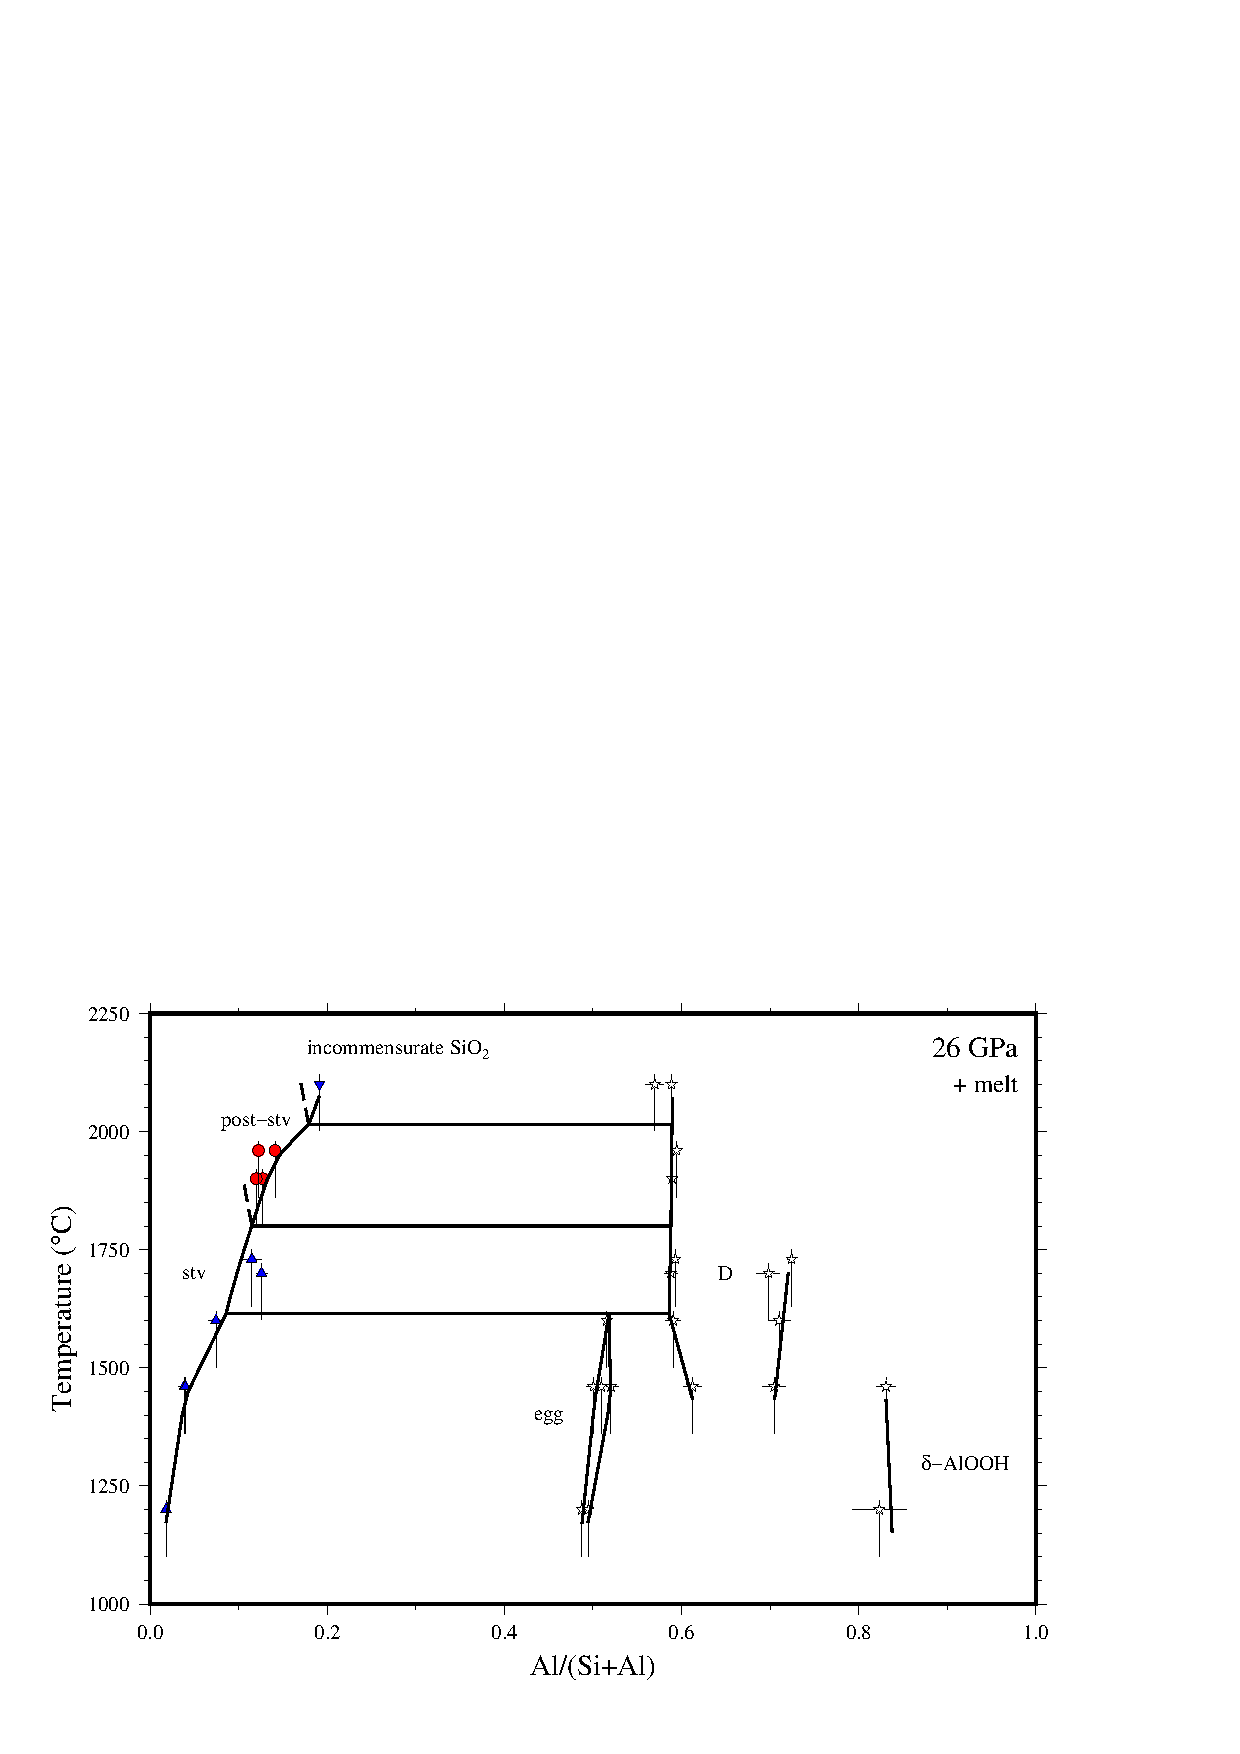
\includegraphics[width=1.0\textwidth]{figures/phase_diagram.pdf}
  \caption{SiO$_2$--AlOOH pseudobinary phase diagram at 26 GPa, based on experimental data \citep{Pamatoetal2015}. Solid phases are in equilibrium with a water-rich melt.}
  \label{fig:phase_diagram}
\end{figure}

\clearpage
\section{Methods}
\subsection{Experimental methods}
The starting compositions for the synthesis of post-stishovite are SiO$_2$ and Al(OH)$_3$, mixed to achieve Al:Si ratios of 1:9 and 3:17. The reagents were first dried, then weighed in the required proportions and ground under ethanol. The powdered samples were loaded into platinum capsules that were sealed by arc welding. Capsules were made of 1 mm outer diameter platinum tubing and had initial lengths of 1.0--1.2 mm. High pressure experiments were carried out using 1200t and 1000t 6-8 Kawai type multianvil apparatuses at the Bayerisches Geoinstitut (BGI). 7 mm edge length Cr$_2$O$_3$-doped MgO octahedra were used as pressure media in combination with tungsten carbide cubes of 32 mm edge length and 3 mm truncation edge length (7/3 assembly). In this type of assembly, the LaCrO$_3$ tube was placed directly into the octahedron and no insulting ZrO$_2$ sleeves were used (due to the reduced space in the assembly). The temperature was measured using W3\%Re/W25\%Re (type D) thermocouple wires (0.13 mm thick) inserted longitudinally through the wall of the heater, with the hot junction at the center of the assembly. The pressure calibration used in this study is reported in the literature \citep{KF2005}. After heating at high pressure, the experiments were quenched by shutting off the power. Short heating durations were chosen to limit water loss. The samples were recovered after a 15 hour decompression phase.

\subsection{Analysis}
\paragraph{a. SEM/EBSD}
The run products were characterized using a GEMINI LEO (now Zeiss) 1530 scanning electron microscope operating at 20 kV accelerating voltage, a beam current of about 2 nA and a working distance of 14 mm. 

\paragraph{b. EPMA}
The chemical compositions of the run products were measured with a JEOL JXA-8200 electron probe microanalyser operating at 20 kV and 20 nA. The beam current caused only minor damage to the phases. The electron beam size was approximately 1-2 $\mu$m in diameter and the peak counting times were 20 s. The concentrations of Si and Al were determined using diopside and pyrope as standards.

\paragraph{c. ERDA}
For accurate determination of water contents, we mirror polished the sample chambers without heat or water, and then mounted them in indium. Elastic recoil detection analysis (ERDA) was conducted in Saclay, Paris. This technique works by bombarding the sample with $^4$He accelerated by a 3 MeV van der Graaff generator at a 15$^{\circ}$ angle to the surface. Hydrogen atoms are removed from the top layers of the sample, and then recorded by an elastic recoil detector. Major/minor and trace element (Z>15) concentrations are estimated via Rutherford backscatter (RBS) and Particle induced X-ray emission (PIXE) detectors. The incident beam is sufficiently high energy that the probability of hydrogen ejection is not dependent on the characteristics of the lattice, making ERDA a powerful tools for estimating hydrogen concentrations in the absence of suitable calibrations. Furthermore, although ERDA probes the surface of the sample, there is some depth resolution, allowing the user to remove the effect of contaminated surface layers. Finally, as the elastic recoil detector can detect a very high proportion of hydrogen atoms ejected from the surface, the process is essentially non-destructive. Full details of the sample preparation and analytical technique can be found in \citep{WBRH2012}.

\paragraph{d. XRD}
Experimental runs performed at lower temperatures and pressures resulted in a fine grained powder. For phase identification of these run products, powder X-ray diffraction patterns were collected using a PHILIPS Xpert diffractometer, operating at 40 kV and 40 mA with CoK$\alpha$ radiation ($\lambda$=1.78897 \AA). Diffraction patterns were collected in the 2$\Theta$ range from 15$^{\circ}$ to 90$^{\circ}$. Phase identification was carried out using the WinXPow Stoe program.


\paragraph{e. TEM}
The samples were prepared for TEM investigation by crushing crystal fragments between two glass slides. The powdered samples were then dispersed in ethanol and loaded on a Lacey carbon TEM grid. The samples were studied using an analytical transmission electron microscope (ATEM, Philips CM-20FEG) operating at 200 kV. The crystals were characterised by selected area electron diffraction (SAED), bright-field (BF) imaging and EDXS spectra, collected using an energy dispersive X-ray spectrometer (NORAN Ge detector).

\paragraph{f. Raman spectroscopy}
Raman spectroscopy was performed on a single-crystal of stishovite (from sample H4095a) with a Dilor XY system. The system was operated with a 514 nm Ar$^+$ ion laser and a liquid nitrogen-cooled CCD detector. The resulting spectrum can be compared to pure stishovite and $\delta$-AlOOH. 


\clearpage
\section{Results}
The experimental run conditions and chemical compositions of the synthesised post-stishovite crystals are shown in Table \ref{tab:results}. The polished capsules revealed elongate crystals of an SiO$_2$-rich phase up to 0.3 mm in length. In the samples with Al:Si ratios of 3:17, a small fraction of a secondary phase was observed at the cold end of the capsule (Figure \ref{fig:sem}). Compositions of these phases estimated by EPMA and ERDA are consistent with stishovite/post-stishovite and phase D, as expected from previous experiments by \cite{Pamatoetal2015}.

\begin{table}[ht!]
\centering
\caption{Experimental conditions for experiments run at 26 GPa and alumina and water contents determined by EPMA and ERDA. RT is the ERDA run time. The two analyses in H4095a correspond to different regions.}
\label{tab:results}
\begin{tabular}{llllllll}
  Expt. \# & T ($^{\circ}$C) & t (min) & RT (min) & Al$_2$O$_3$ (wt \%) & H$_2$O (wt \%) & H/Al        & Coexisting phases \\
  \hline
  S6239a   & 1900  & 5  & 67 & 10.1 +/- 0.2  & 2.0 +/- 0.3 & 1.3 +/- 0.2 &                   \\
  S6239b   & 1900  & 5  & 60 & 10.9 +/- 0.3  & 2.5 +/- 0.3 & 1.3 +/- 0.2 & Phase D           \\
  H4095a1  & 1960  & 15 & 41 & 10.3 +/- 0.4  & 2.0 +/- 0.3 & 1.1 +/- 0.2 &                   \\
  H4095a2  & 1960  & 15 & 20 & 10.3 +/- 0.4  & 2.0 +/- 0.3 & 1.1 +/- 0.2 &                   \\
  H4095b   & 1960  & 15 & 60 & 12.1 +/- 0.1  & 2.3 +/- 0.3 & 1.1 +/- 0.2 & Phase D          
\end{tabular}
\end{table}


\begin{figure}[ht!]
  \centering
  \includegraphics[width=1.0\textwidth]{figures/H4095b.pdf}
  \caption{Back scattered electron image of sample H4095b. Light grey regions are large single crystals of stishovite. Darker grey is Phase D, which has crystallised at the cold end of the capsule. Stishovite at the cold end of the capsule has lower Al-contents ($\sim$11.7 wt \%) which are not included in the average given in Table \ref{tab:results}.}
  \label{fig:sem}
\end{figure}

X-ray powder diffraction of all four samples revealed broadening or splitting of (hkl) peaks where h$\neq$k, diagnostic of the post-stishovite phase (e.g. Figure \ref{fig:xrd}). A single crystal structural refinement yielded an accurate estimate of the unit cell parameters of post-stishovite with 10 wt \% Al$_2$O$_3$ (Figure \ref{fig:volumes}).
\begin{figure}[ht!]
  \centering
  \includegraphics[width=1.0\textwidth]{figures/stv_xrd_comparison.pdf}
  \caption{Powder XRD analysis of sample H4095a compared with pure stishovite}
  \label{fig:xrd}
\end{figure}


The water contents of our synthesised crystals are compared with literature values in Figure \ref{fig:water_contents}. Water contents in stishovites estimated from FTIR calibrations are generally 10--30\% of those expected from Al and H substituting for Si, and require significant Al to be charge balanced by oxygeen defects. In contrast, our results for post-stishovite can be explained almost completely by the Si $\rightarrow$ Al + H substitution. In the case of S6239, it may even be necessary to invoke a hydrogrossular-type substitution (Si $\rightarrow$ 4 H). Deficits in EPMA totals suggest that the hydrous phase D reported by \cite{Pamatoetal2015} may also be more water rich than the SiO$_2$-AlOOH binary, although we are wary of drawing strong conclusions from electron probe deficits on dense hydrous magnesium silicates.

\begin{figure}[ht!]
  \centering
  \includegraphics[width=1.0\textwidth]{figures/stv_water_contents.pdf}
  \caption{Aluminium and water contents for stishovites analysed in \cite{LLSHLOB2007} via two FTIR calibrations and in this study by ERDA.}
  \label{fig:water_contents}
\end{figure}


TEM analysis revealed no secondary phase inclusions which could affect water contents estimated by ERDA, even in capsules which exhibited phase D crystallisation (Figure \ref{fig:tem}). This clearly indicates that run durations and temperatures were sufficiently high to allow phase separation. This is in clear contrast to syntheses of bridgmanite, which commonly exhibit inclusions of dense hydrous magnesium silicates which can result in erroneously high water estimates \citep{KB2006}.  

Raman spectroscopy reveals an extremely prominent set of absorption peaks at 1850-1960 cm$^{-1}$ (Figure \ref{fig:raman}). These peaks are larger than the principal peaks at 220 cm$^{-1}$ and 750 cm$^{-1}$. The frequency-bond length relation proposed by \cite{Libowitzky1999} indicates strong hydrogen bonds in post-stishovite, with $d$(O$\cdot\cdot\cdot$O)=2.62--2.64 \AA\ and $d$(H$\cdot\cdot\cdot$O)=1.66--1.69 \AA. The H$\cdot\cdot\cdot$O bond length is comparable with that estimated from the ab-initio estimates of \cite{PS2004} (1.694 \AA\ and 1.21 \AA\ for 4.2 and 100 mol \% AlOOH, linearly interpolated as  1.654 \AA\ at 12 mol\% AlOOH).

\begin{figure}[ht!]
  \centering
  \includegraphics[width=1.0\textwidth]{figures/ambient_stv_cell_parameters.pdf}
  \caption{Stishovite and post-stishovite unit cell parameters}
  \label{fig:volumes}
\end{figure}

\begin{figure}[ht!]
  \centering
  \includegraphics[width=1.0\textwidth]{figures/H4095b_stv_TEM_darkfield_w_saed.pdf}
  \caption{Darkfield TEM image with selected area electron diffraction (SAED) of sample H4095b.}
  \label{fig:tem}
\end{figure}

\begin{figure}[ht!]
  \centering
  \includegraphics[width=1.0\textwidth]{figures/raman.pdf}
  \caption{Raman spectra of hydrous aluminous stishovite bearing 2 wt \% H$_2$O. The overlapping large amplitude peaks at 2850--2960 cm$^{-1}$ indicate strong hydrogen bonding \citep{Libowitzky1999}. Raman spectra of pure stishovite \citep{RRUFF}, $\delta$-AlOOH \citep{XKFIH2006} and phase D \citep{Pamatoetal2015} are provided for comparison. Different normalisations are used for the high and low wavenumber parts of the $\delta$-AlOOH and phase D spectra.}
  \label{fig:raman}
\end{figure}

\clearpage

\section{Discussion}
\subsection{Transition pressure}
This study confirms and extends previous work showing that the incorporation of aluminium and hydrogen into SiO$_2$ lowers the stishovite$\rightarrow$post-stishovite transition pressure. This is in agreement with ab-initio results, which suggest that the incorporation of interstitial hydrogen plays an important role in reducing the transition pressure by relieving the mismatch between Al-O and Si-O bond lengths, and therefore allowing rotation of the Al-octahedra \citep{PS2004,UKHRW2015}.

It has been argued that aluminium under anhydrous conditions can also reduce the stishovite-post-stishovite transition pressure by inducing a `chemical pressure' \citep{BAAG2009}. However, the `chemical pressure' imposed by aluminium should be negative, decreasing distortion of the octahedral cation site and inhibiting octahedral rotation \citep{SSP1995, UKHRW2015}. The addition of Al should therefore have little effect on the stishovite-post-stishovite transition \citep{Panero2006}. The results of \cite{BAAG2009} are therefore unexpected; it seems possible that another component (such as H$_2$O) or deviatoric stress acted to stabilise the CaCl$_2$ structure.

Another unexpected result of \cite{BAAG2009} was the successful decompression of post-stishovite (Sample Sti-06) synthesised from material with 4 wt \% SiO$_2$. The reported cell parameters of this sample are remarkably similar to our results for material with 10 wt \% SiO$_2$ (Figure \ref{fig:volumes}).



\subsection{Water in the lower mantle}
Water capacities in the upper mantle generally increase with depth, and the mantle transition zone can contain about 1 wt \% H$_2$O \citep{KB2006}. In the lower mantle, water capacities are much more controversial. Mg-bridgmanite and periclase probably contain $>$20 ppm H$_2$O under uppermost lower mantle conditions, although the effect of Fe, Al and pressure on H$_2$O incorporation in bridgmanite has yet to be fully investigated. Water contents in Ca-perovskite are difficult to analyse, given the amorphisation of Ca-perovskite during decompression/analysis. Finally, the recent discovery of hydrous Phase H \citep{NITTNFH2014, BNTI2014, OAKSH2014} and its solid solution with $\delta$-AlOOH \citep{OOSMHON2014} has raised the possibility of large amounts of water in all but the lowermost mantle \cite{Ohtani2015}. However, careful diamond anvil cell experiments on the stability of this new phase suggest that hydrous phase stability may be limited to subducting slabs \citep{Walteretal2015}.

In this study, we have synthesised post-stishovites with hydroxyl concentrations consistent with an SiO$_2$-AlOOH solid solution. This is equivalent to approximately 0.5-0.9 wt\% H$_2$O in stishovite with 3--5 wt\% Al$_2$O$_3$. These water solubilities are approximately 5-7 times higher than in stishovite \citep{LKSOLBI2007, CK2002}. The simplest explanation is that pressure promotes the accommodation of interstitial hydrogen. This is consistent with the estimated volumes of post-stishovite, which are smaller than the linear extrapolations of stishovite. It is also consistent with the structural conclusions of ab-initio data, which suggest that hydrogen incorporation promotes Al-octahedral rotation \citep{PS2004}. The inferred bond lengths from \cite{Libowitzky1999} suggest that hydrogen bonding in post-stishovite is strong but asymmetric, also in agreement with the ab-initio results.

The increasing preference for AlOOH incorporation into SiO$_2$ over Al incorporation via the formation of oxygen vacancies suggests that stishovites will become increasingly undersaturated in water during subduction. In the lower mantle, hydrous melts will react with water-undersaturated post-stishovites, providing a mechanism for the migration of water from ultramafic to mafic rocks as proposed for Phase D by \cite{Pamatoetal2015}. This percolation and reaction may explain the patchy nature of low velocity layers in the uppermost lower mantle \citep{SJBLD2014}. Unlike Phase D and other hydrous phases, post-stishovite is extremely stable both as a function of pressure and temperature, and is thus a more natural potential host for water in the deep convecting mantle.


One further interesting possibility is that the breakdown of post-stishovite in the lowermost mantle may cause melting and an explanation for ULVZs at the core-mantle boundary. Post-stishovite undergoes a phase transition to the mineral seifertite with the scrutinyite ($\alpha$-PbO$_2$) structure (orthorhombic, Pbcn, no. 60) \citep{MHOO2003, GSP2013} at 120--140 GPa. There are no simple hydrous phases known with the seifertite structure, and very low saturated water contents in the isostructural TiO$_2$ (II) phase \citep{BHM2004} suggest that this phase may be essentially dry. Any mafic material passing through the post-stishovite $\rightarrow$ seifertite phase boundary will create a hydrous partial melt, which is then likely to percolate towards the core-mantle boundary.



\subsection{Seismic scattering in the lower mantle}
Seismic reflections have been observed in the lower mantle at a variety of depths, from 700 to 1200 km \citep[e.g.][]{DAD2013}. The stishovite to post-stishovite transition has become an important candidate for these scattered phases \citep{BSBIWJ2010,AHOHOM2013,BR2014}, which in pure SiO$_2$ would occur at approximately 1700 km depth \citep{HTSO2005,Nomuraetal2010}. The addition of alumina provides an ideal mechanism to reduce the depth of the transition \citep{Lakshtanovetal2007}. If water is also required, as suggested by structural and ab-initio studies \citep{SSP1995,PS2004,UKHRW2015} then the scattering also provides an indication of locations of hydrated rocks in the lower mantle. However, we caution that it is the second order nature of the SiO$_2$ transition which leads to the shear modulus reduction \citep{CHM2000}. If hydrogen plays a key role in the symmetry breaking, then the transition in hydrated aluminous stishovites may no longer be first order \cite{UKHRW2015}. If the stishovite-post-stishovite transformation is to blame for the scattering, other mechanisms for shear modulus reduction must be important, such as anelasticity resulting from hydrogen mobility at seismic frequencies \citep[termed Snoek relaxation;][]{Snoek1941, NB1972, MCDBT2007, UKHRW2015}.


%\cite{KH1998,KH2003} \cite{NKF2003} \cite{KBSW2001} \cite{Kaneshima2009} \cite{BSBIWJ2010} \cite{KHSBIWJ2010}   \cite{Mookherjee2011}


\section{Conclusions}
In this study, we have shown that the stishovite to post-stishovite reaction is associated with an increased preference for incorporation of hydrogen. This incorporation is strongly correlated with alumina content, and is consistent with a 1:1 substitution of silicon with aluminium on the octahedral site, charge balanced by interstitial hydrogen. Post-stishovites in the lower mantle may contain 0.5--0.9 wt\% H$_2$O, allowing them to soak up water released by the breakdown of other water-bearing phases. In the absence of hydrous phases, which become unstable at temperatures similar to typical mantle geotherms \citep{Walteretal2015}, post-stishovite may be the primary water-bearing phase in the lower mantle.


\clearpage


\section{Supplementary materials}


\begin{figure}[ht!]
  \centering
  \includegraphics[width=1.0\textwidth]{figures/s6239_long_rrp.pdf}
  \caption{Structure}
  \label{fig:structure}
\end{figure}

\clearpage
\section*{References}

\bibliography{references_stv}

\end{document}
